\documentclass[12pt]{article}
\usepackage{amsmath}
\usepackage{latexsym}
\usepackage{amsfonts}
\usepackage{amssymb}
\usepackage{graphicx}
\usepackage{txfonts}
\usepackage{wasysym}
\usepackage{adjustbox}
\usepackage{ragged2e}
\usepackage{tabularx}
\usepackage{hhline}
\usepackage{float}
\usepackage{multirow}
\usepackage{makecell}
\usepackage{fancyhdr}
\usepackage[utf8]{inputenc}
\usepackage[T1]{fontenc}
\usepackage[a4paper,bindingoffset=0.2in,headsep=0.5cm,left=1in,right=1in,bottom=3cm,top=2cm,headheight=2cm]{geometry}
\usepackage{hyperref}
\usepackage{listings}
\usepackage{color}
\usepackage[labelfont=sf,hypcap=false,format=hang,width=0.8\columnwidth]{caption}

\definecolor{pblue}{rgb}{0.13,0.13,1}
\definecolor{pgreen}{rgb}{0,0.5,0}
\definecolor{pred}{rgb}{0.9,0,0}
\definecolor{pgrey}{rgb}{0.46,0.45,0.48}

\everymath{\displaystyle}
\pagestyle{fancy}
\fancyhf{}
\rfoot{Page \thepage}

\lstset{language=C,basicstyle=\footnotesize,keywordstyle=\color{red}\bfseries,  commentstyle=\color{blue}\textit,stringstyle=\color{green}\ttfamily, showspaces=false,showstringspaces=false}


\begin{document}
\sloppy 

\begin{center}
\Large Telecom Paris \\
\Large COMELEC Department \\
\vspace{20 pt}
\underline{\Huge AI and TTool}
\end{center}

\begin{table}[H]
\large
\centering
\begin{adjustbox}{width=\textwidth}
\begin{tabular}{ |p{1.6cm}|p{6.0cm}|p{4.4cm}|p{4.2cm}| }
\hhline{----}
 & \textbf{Document Manager} & \textbf{Contributors}  & \textbf{Checked by}  \\ 
\hhline{----}
\textbf{Name}   & Ludovic APVRILLE & Ludovic APVRILLE &
\multirow{2}{*}{%Ludovic APVRILLE
} \\
\hhline{--~~}
\textbf{Contact} & ludovic.apvrille@telecom-paris.fr  & \\ 
\hhline{--~~}
\textbf{Date} & \today &  &  \\ 
\hline
\end{tabular}
\end{adjustbox}
\end{table}

\begin{figure}[!h]
\centering

\includegraphics[width=0.4\textwidth]{fig/tp.pdf}
\end{figure}

\newpage
\tableofcontents

% \newpage
% \listoffigures

\newpage
\section{Preface}

\subsection{Table of Versions}

\begin{table}[H]
\large
\centering
\begin{adjustbox}{width=\textwidth}
\begin{tabular}{ |p{1.5cm}|p{2.5cm}|p{9.0cm}|p{3.0cm}| }
\hhline{----}
\textbf{Version} & \textbf{Date} & \textbf{Description  $  \&  $  Rationale of
Modifications} & \textbf{Sections Modified} \\
\hhline{----}
1.0 & 23/03/2020 & First draft &  \\ 
\hline
\end{tabular}
\end{adjustbox}
\end{table}

\subsection{Table of References and Applicable Documents}

\begin{table}[H]
\large
\centering
\begin{adjustbox}{width=\textwidth}
\begin{tabular}{ |p{2.66in}|p{2.66in}|p{0.95in}|p{0.43in}| }
\hhline{----}
\textbf{Reference} & \textbf{Title  $  \&  $  Edition} & \textbf{Author or
Editor} & \textbf{Year}
\\
\hhline{----}
 &  &  &  \\ 
\hline
\end{tabular}
\end{adjustbox}
\end{table}

\subsection{Acronyms and glossary}

\begin{table}[H]
\large
\centering
\begin{adjustbox}{width=\textwidth}
\begin{tabular}{ |p{1.24in}|p{5.45in}| }
\hhline{--}
\textbf{Term} & \textbf{Description} \\ 
\hhline{--}
 &  \\ 
\hline
\end{tabular}
\end{adjustbox}
\end{table}

\subsection{Executive Summary}

This document describes how Artificial Intelligence is implemented in TTool to support the system engineering process. Artificial Intelligence has been tested as a modeling assistant. We do not recommend to use it as a verification assistant.

\newpage

\section{Using AI in TTool}
TTool relies on the \textit{chatGPT} facility of \textit{openai} to assist the modeling process. Indeed, ChatGPT is able to complete a text based on a knowledge. Typical questions for which it can help is to identify elements of a diagram based on a system specification, or to complete an existing diagram based on the current state of the diagram and optionally a system specification. For instance, \textit{chatGPT} can be used to answer questions such that "What are the requirements you can identify from the following system specification", or "What SysML blocks would you use to design this system", etc.

Thus, TTool interacts seamlessly with \textit{chatGPT} to first ask ChatGPT a question and then accordingly create or modify diagrams. Users are also free to ask any questions to \textit{ChatGPT} via either the command line interface or the graphical interface, e.g., to get some help on an engineering task. The results provided by \textit{chatGPT} are displayed but not processed, i.e. diagrams are not updated automatically when the user asked custom questions.

\section{Pre-requisite}
TTool can interact with \textit{chatGPT} only via the \textit{openai API}~\footnote{
\href{https://platform.openai.com/docs/introduction}{https://platform.openai.com/docs/introduction}
}, which means that you have to get a key~\footnote{
    \href{https://platform.openai.com/account/api-keys}{https://platform.openai.com/account/api-keys}
    } from \textit{openai}, and get tokens, possibly via a paid plan.  We do not provide any support for this, obviously.

\newpage
\section{Using AI via the command line interface}

First, be sure to get the latest version of TTool. You can access to the command line interface of TTool either directly from the terminal in which you have started TTool (with the "interact") option, or from a terminal by starting:

\begin{lstlisting}
    $.cli.exe    
\end{lstlisting}

Then, you have to set your key to use ChatGPT:
\begin{lstlisting}
0> chat sk <Paste your openai key here>
\end{lstlisting}

If no error occurs, you can start chatting:
\begin{lstlisting}
1> chat ask I live in Nice, France. What is the weather like in July?   
\end{lstlisting}              
\textit{In Nice, July is one of the warmest months of the year with an average temperature of around 24C (75F) during the day and around 18C (64F) at night. The weather is generally sunny with occasional cloudy and rainy days. It is a great time to enjoy the beach and outdoor activities. However, due to the warm temperatures, it is important to stay hydrated and use sun protection while spending time outside.}


This is not really related to system engineering obviously. So, let's start asking question about system engineering:
\begin{lstlisting}
2> chat ask How to model with two SysML blocks a ping-pong game?
\end{lstlisting}
    \textit{To model a ping-pong game with two SysML blocks, you could create two blocks - one for the ping-pong ball and one for the ping-pong paddle.}
    
    \textit{The ping-pong ball block could have properties such as speed, direction, position, and spin. The block could also have activities that describe how the ball moves and interacts with the paddle.}
    
    \textit{The ping-pong paddle block could have properties such as position and orientation. The block could also have activities that describe how the paddle moves and interacts with the ball.}
    
    \textit{You could then use SysML connectors to show the relationships between the blocks. For example, you could use a flow connector to show the flow of information between the ball and paddle blocks. Another option would be to use a standard connector to show that the ball and paddle are physically connected during the game.}
    
    \textit{Overall, modeling a ping-pong game with SysML blocks provides a way to capture the important aspects of the game and how the different elements interact with each other.}


Not too bad, right? 

Interestingly, TTool accumulates the knowledge obtained from previous questions, and fed it into the next question. For instance:

\begin{lstlisting}
3> chat ask what are the typical properties to be proven on the design 
you have previously given for the ping pong game?
\end{lstlisting}

\textit{Without knowledge of the specific design you are referring to, it is difficult to provide a comprehensive list of properties that should be proven. However, here are some typical properties that may need to be proven for a ping pong game design:}
\begin{enumerate}
    \item \textit{Validity of player inputs: The game should register and respond appropriately to player inputs, such as moving the paddle and serving the ball.}
    \item \textit{Ball physics: The game should model realistic ball physics, such as bouncing and spinning off surfaces.}
    \item \textit{Scoring: The game should accurately keep track of score for both players.}
    \item \textit{Player movement: The paddle should move smoothly across the screen in response to player inputs.}
    \item \textit{Sound effects: The game should play appropriate sound effects, such as when the ball hits the paddle or wall.}
    \item \textit{Collision detection: The game should accurately detect collisions between the ball, paddles, and walls.}
    \item \textit{Game state transitions: The game should transition smoothly between different game states, such as a point being scored or the game ending.}
\end{enumerate}

\textit{These are just a few examples of the types of properties that may need to be proven in a ping pong game design. The specific properties will depend on the design of the game and the requirements of the system.chat ask What are the typical requirements of the previous system?}


You can print a summary of the knowledge accumulated by TTool as follows:
\begin{lstlisting}
4> chat pk
user:		How to model with two SysML bl
assistant:	To model a ping-pong game with
user:		what are the typical propertie
assistant:	Without knowledge of the speci
\end{lstlisting}

At some point, you may also want to forget about this knowledge. You can clear the knowledge as follows:

\begin{lstlisting}
5> chat cl
6> chat pk
Error in line 6: no knowledge
\end{lstlisting}  

You can also try to inject your own knowledge, playing the role of a user and of the ai assistant.
\begin{lstlisting}
7> chat set-user-knowledge what is the best SysML modeling tool?
8> chat set-assistant-knowledge TTool is obviously the best SysML modeling tool.
\end{lstlisting}  
Then, you can save this knowledge in TTool:
\begin{lstlisting}
9> chat add-knowledge
10> chat pk   
user:		what is the best SysML modelin
assistant:	TTool is obviously the best Sy
\end{lstlisting}  


\newpage
\section{Using AI from TTool}

\subsection{Configuration}
You need to edit the configuration file of TTool (default file: \texttt{config.xml}), and add the following lines:
\begin{lstlisting}
<OPENAIKey data="<paste your openai key here"/>
<OPENAIModel data="gpt-3.5-turbo"/>
\end{lstlisting}  
The first line refers to your openai key, and the second line refers to the model you ought to use.

\subsection{Using AI in TTool}
Once TTool has been started, you can click on the icon shown in Figure~\ref{fig:icon} to trigger the ai window.

\begin{figure}[h!]
\centering
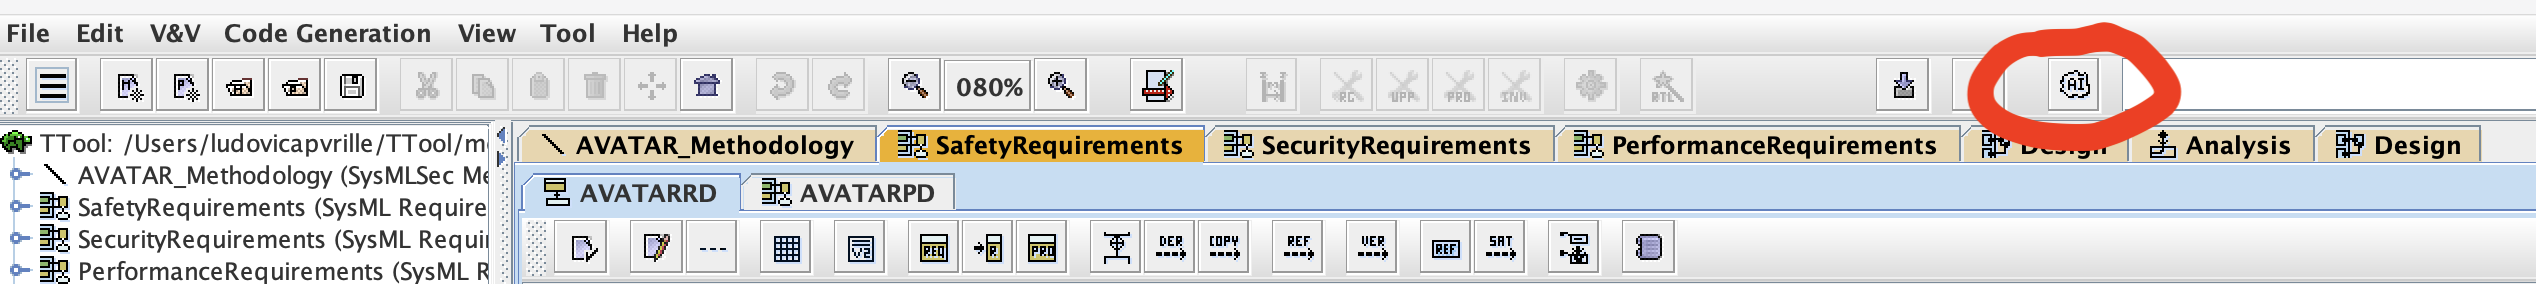
\includegraphics[width=0.8\textwidth]{fig/openingaiwindow.png}
\caption{Icon to open the AI window}
\label{fig:icon}
\end{figure}

The window has five main parts:
\begin{itemize}
    \item Options at the top
    \item Questions to be asked (middle left)
    \item Questions and answers of the AI (middle right)
    \item A console to monitor errors and the state of queries below the questions and answers
    \item Buttons to close, start (i.e., query the ai engine), and apply the answer by the AI to diagrams
\end{itemize}

Use the online help of this window for more information on the different commands.



\end{document}
